% !TeX root = ../main.tex
% Add the above to each chapter to make compiling the PDF easier in some editors.

\chapter{Evaluation}\label{chapter:Evaluation}

The goal of this chapter is to validate the framework architecture design for context-aware pervasive computing in challenged environments which was described in Chapter \ref{chapter:Approach}. It also evaluates the middleware implementation which was explained in Chapter \ref{chapter:implementation}. Note that, the delays and performances are to be taken with a grain of salt, as the system is designed as a proof-of-concept and not to run in production systems. \\

\noindent In order to evaluate the framework and implementation with all its requirements, we divided the evaluation into several use cases. The devices used for  the use cases has different hardware capabilities. They might also have  sensors and actuators according to each use case. All the devices must be running our stack framework as explained in \ref{subsec:starting-framework} except for android phones which has \textit{Liberouter}, an implementation for SCAMPI on android phones. The devices we used in this evaluation are:
\begin{table}[!ht]
	\centering
	\begin{tabular}{*{4}{c}}\toprule
		Name & Count & Stack & Performance \\ \hline
		 &  &  &  \\
		Intel NUC &1& 	Our framework &   \specialcell[c]{CPU:Intel Core i5-6260U Processor\\ (4M Cache, up to 2.90 GHz)\\RAM: 16GB }\\ 
		&  &  &  \\
		Raspberry Pi 3 model B & 2 & Our framework &  \specialcell[c]{ CPU: 1.2GHz\\RAM: 1GB}  \\ 
		&  &  &  \\
		HTC One M9 & 1 & Liberouter &   \specialcell[c]{CPU: Octa-core \\4 x 2.0GHz + 4 x 1.5GHz\\ RAM: 3GB} \\ \hline

\end{tabular}
\caption{Devices used for the implementation evaluation.}
\label{table:devoces}
\end{table}


\section{Recognizing Water Bottles }
This use case detects movements around the low computation devices portrayed as the Raspberry Pis. Once they detect movements around them, they take an image and send it to the topic \textit{NUC}. A high performance machine should be waiting for input on the same topic and as soon as it receives an image, it runs image recognition and responds back to the Raspberry Pi which sent the original message  only if the recognizer found a water bottle. When a Raspberry Pi receives the recognition result on its endpoint, this means that the image was a watter bottle with a certain confidence, therefore, the Pi signals a red led to start and stores the result in a database. The flows implementation used to create this use case can be found in \ref{subsec:tensor} and \ref{subsec:detect-move}. 

\noindent As stated every device must have the framework stack running before we start our use case. So after making sure its running we start publishing the flows. In this use case, the testbed setup is shown in figure \ref{fig:tb-tensor}, it consists of two Raspberry Pis, an Intel NUC and a router connected via switch. The PC which will publish the computations is connected through the router via WI-FI. 
 \begin{figure}[H]
	\centering
	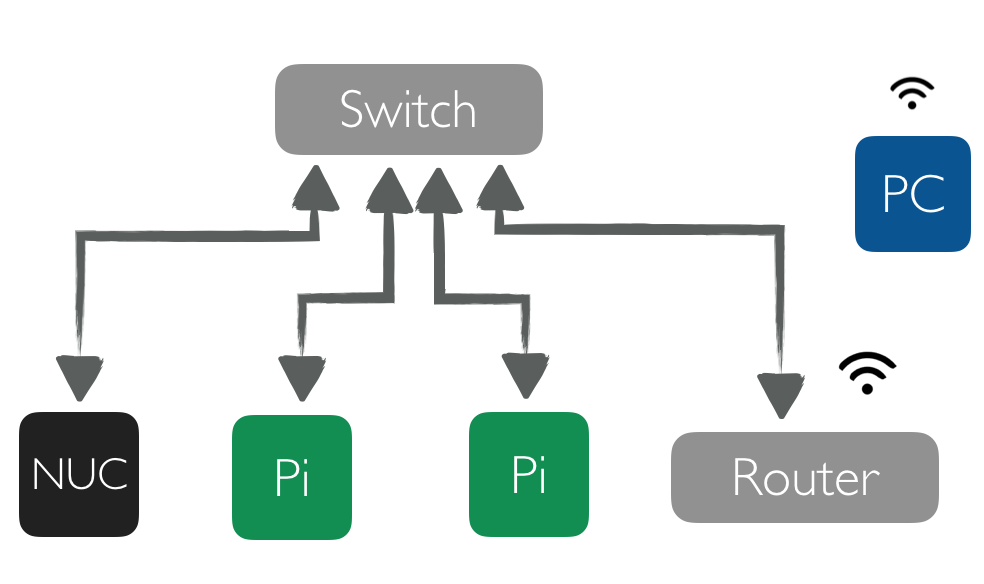
\includegraphics[scale=0.6]{images/tb-tensor.png}
	\caption{Testbed setup for recognizing water bottles.}
	\label{fig:tb-tensor}
\end{figure} 

\noindent We started by publishing the flow \ref{subsec:tensor} for  image recognition with all its dependencies in total 83MB, then we published the motion detection flow \ref{subsec:detect-move} with the sensor scripts. We measured the delay between publishing flows from the PC till it was received and deployed by node-RED on each instance. The use case was run 8 times and all the results can be found in \ref{app:tensor}. We also measured the delay when a motion was detected by Raspberry Pi and an image was sent to the NUC and the recognizer reply, this was also run 8 times for each Pi, a total of 16 runs. The sequence \ref{fig:sd-tensor} diagram illustrates the procedure in addition to the time initials for each part of the process.  
\begin{figure}[H]
	\centering
	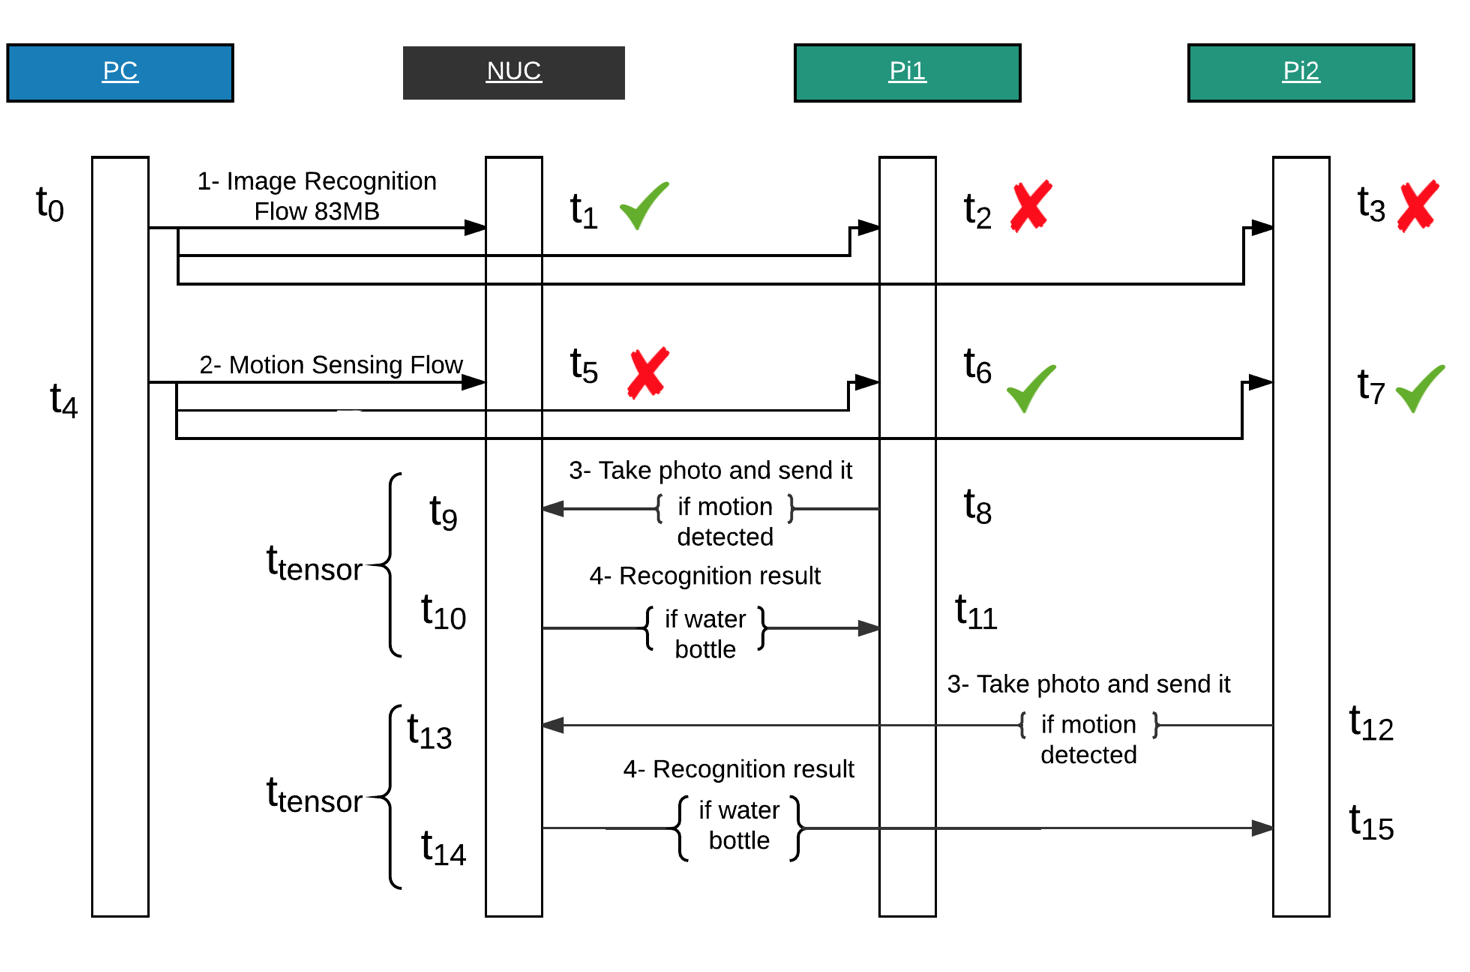
\includegraphics[scale=0.45]{images/sequence-diagram.png}
	\caption{Sequence diagram for recognizing water bottles.}
	\label{fig:sd-tensor}
\end{figure} 

\noindent At time $t_0$ the image recognition flow was published, at times $t_1, t_2, t_3$ it was received by the NUC, Pi1 and Pi2 respectively. Then at time $t_4$ the motion sensing flow was published and at times $t_5,t_6,t_7$ it was received by the other devices as well. A times $t_8,t_{12}$  the Pis detected motion, took an image and then sent a message to the NUC. At times $t9,t{13}$,  NUC received messages from the Pis and started processing, detected a watter bottle and then results were published to the senders at $t_{10},t_{14}$ and received at $t_{11}$ and $t_{12}$. We give the average delay and the standard deviation of the 8 runs in the next tables.
\begin{table}[!ht]
\centering
\begin{tabular}{*{4}{c}}\toprule
&$t_1 - t_0$  & $t_2 - t_0$  & $t_3-t_0$ \\ \midrule
$\Delta t$&	23.245 s&28.226 s&20.826 s\\ 
$\sigma	t$ &1.440 s&8.830 s&8.851 s\\
\end{tabular}
\caption{Mean and standard deviation of the image recognition flow.}
\label{table:tensor}
\end{table}


\begin{table}[!ht]
\centering
\begin{tabular}{*{4}{c}}\toprule
&$t_5 - t_4$  & $t_6 - t_4$  & $t_7-t_4$ \\ \midrule
$\Delta t$ &0.087 s&2.322 s&1.948 s\\
$\sigma t$&0.012 s&0.053 s&0.491 s\\
\end{tabular}
\caption{Mean and standard deviation of the motion detection flow.}
\label{table:motion}
\end{table}

\begin{table}[!ht]
\centering
\begin{tabular}{ c | c | c| c | c| c }	\toprule
&$t_9 - t_8$  & $t_{11} - t_{10}$  & $t_{13}-t_{12}$ & $t_{15}-t_{14}$&  $t_{tensor}$ \\ \midrule
$\Delta t$&0.282 s&0.700 s&	0.273 s&0.6985 s&5.512 s\\
$\sigma t$&0.061 s&0.067 s&	0.048 s&0.0488 s&0.217 s\\
	\end{tabular}
	\caption{Mean and standard deviation for sending and receiving data.}
	\label{table:data}
\end{table}


\section{Challenged Networks}
\begin{figure}[H]
	\centering
	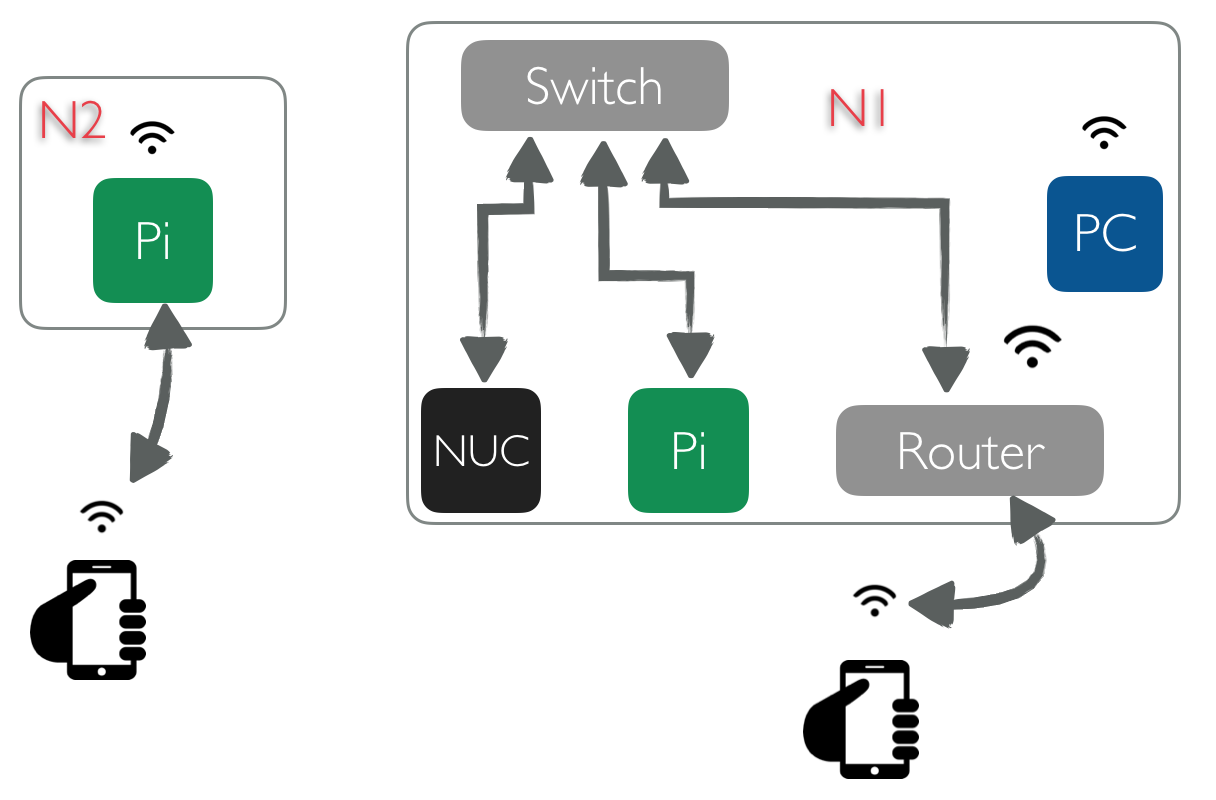
\includegraphics[scale=0.6]{images/tb-dtn.png}
	\caption{Testbed setup for challenged and delay tolerant networks.}
	\label{fig:tb-dtn}
\end{figure} 

\section{Basic IoT Usage}


